%!TEX root = ../Thesis.tex
%\chapter{Long chapter title with $\pi$ $π$ or π}
%\chapter{Long chapter title with \texorpdfstring{$\pi$ $π$ or π}{π π or π}}
\section{Information Theory Considerations in Patch-based Training of Deep Neural Networks on Seismic Time-Series}

\paragraph{Abstract:} Recent advances in machine learning relies on convolutional deep neural networks. These are often trained on cropped image patches. Pertaining to non-stationary seismic signals this may introduce low frequency noise and non-generalizability.
\vfill
\subsection*{Key points:}
\begin{itemize}
    \item \aclp{cnn} use windowed convolutions
    \item Non-stationary data can "seem" offset from zero
    \item Results in erroneous bias within network
\end{itemize}
\vfill
{\vfill\hfill\newline\fbox{\parbox{.97\textwidth}{\fullcite{dramsch2018information}}}}

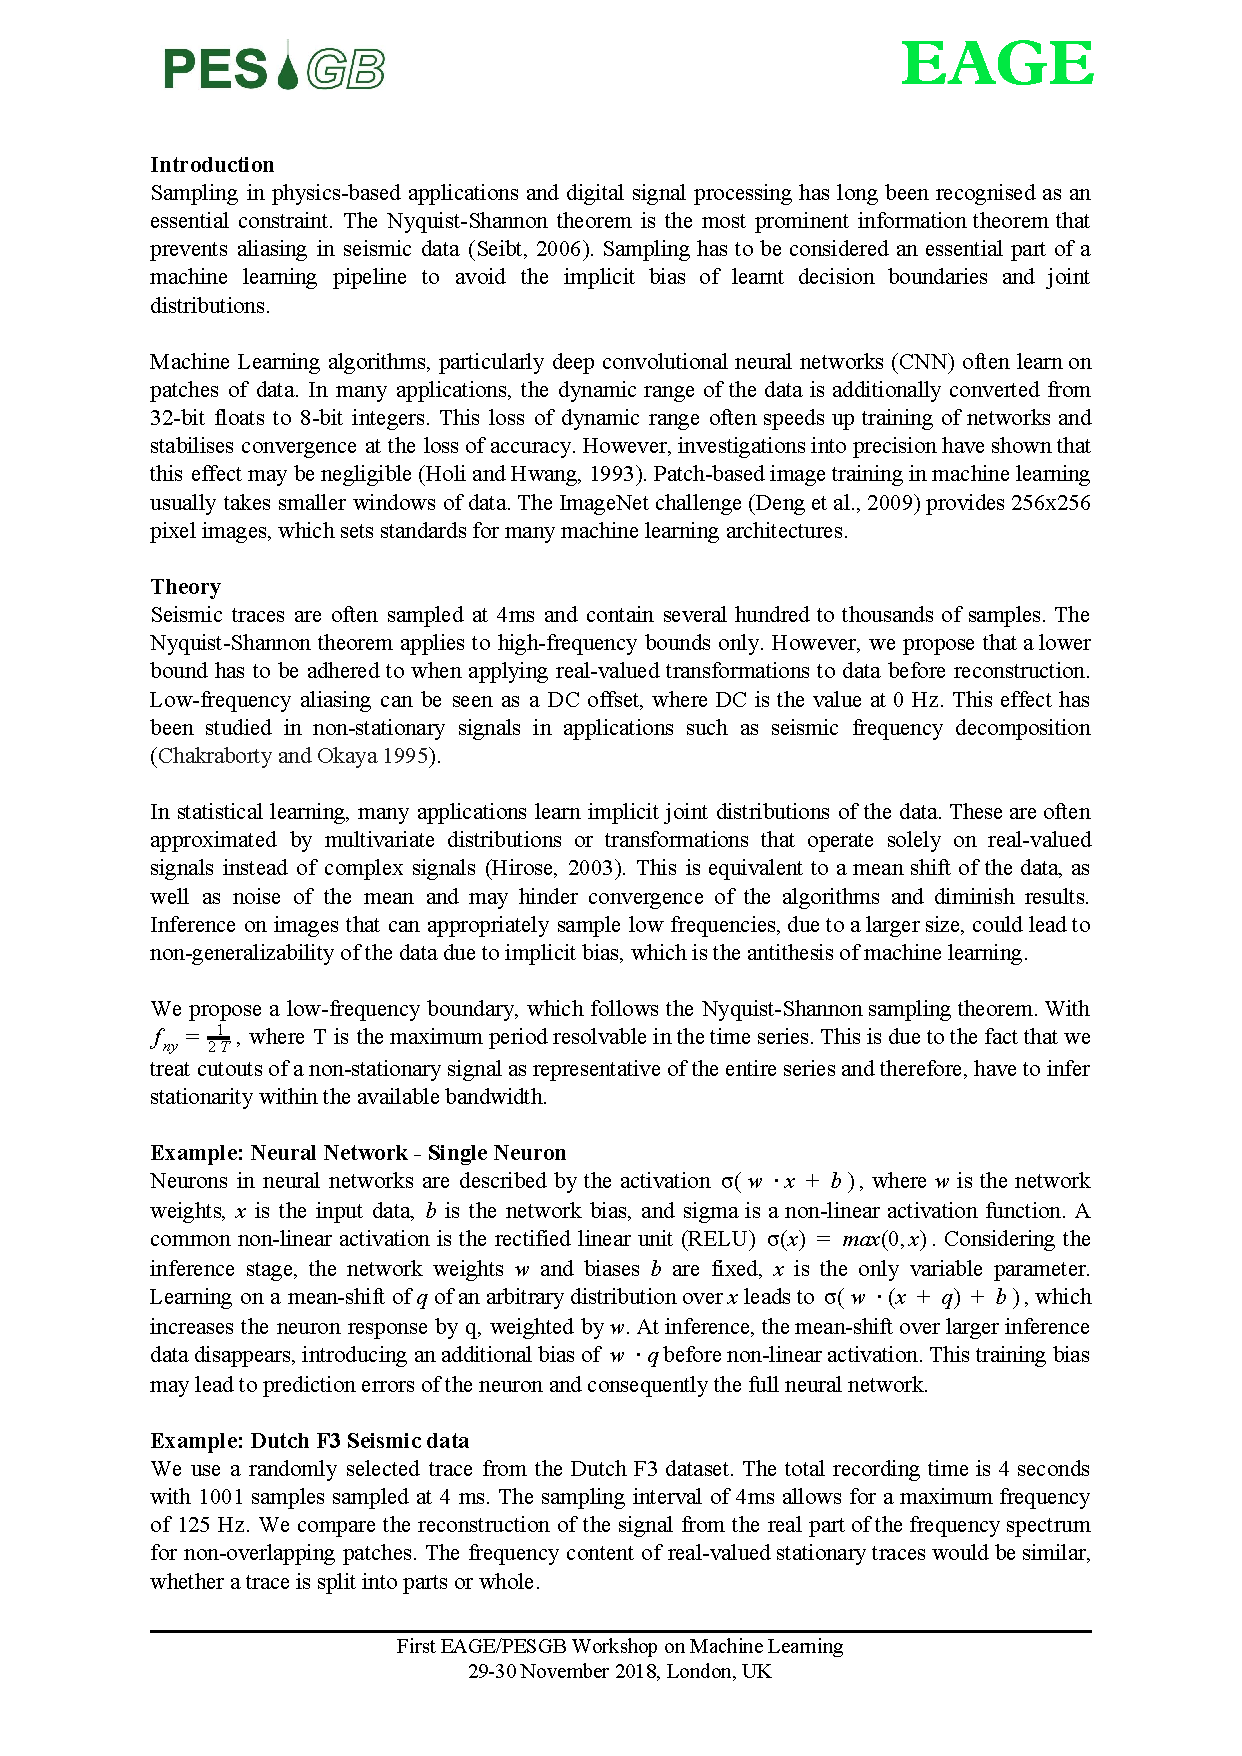
\includepdf[pages={1-2},pagecommand={},width=1.2\textwidth,offset=0.7cm -1.5cm]{papers/2018.3}
